\documentclass{standalone}
\usepackage{tikz}

\usetikzlibrary{calc,shadows}


\begin{document}

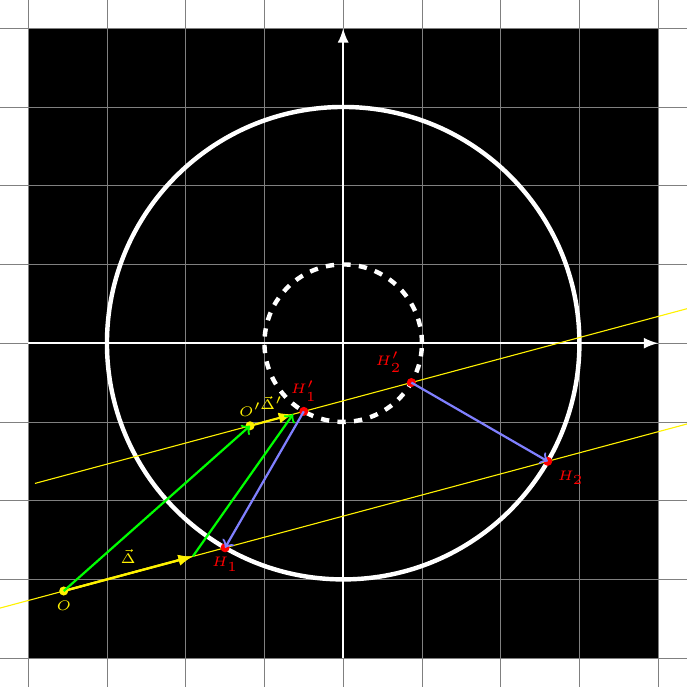
\begin{tikzpicture}
  \draw[fill=black,use as bounding box] (-4,-4) rectangle (4,4);
  \draw[help lines] (-5,-5) grid (5,5);
  \draw[white,-latex,thick] (-4,0) -- (4,0);
  \draw[white,-latex,thick] (0,-4) -- (0,4);

  \draw[white,ultra thick] (0,0) circle [radius=3cm];
  \draw[white,ultra thick,dashed] (0,0) circle [radius=1cm];

  \coordinate (small hit 1) at (-120:1);
  \coordinate (small hit 2) at (-30:1);
  \coordinate (big hit 1) at (-120:3);
  \coordinate (big hit 2) at (-30:3);
  \coordinate (small ray origin) at ($ (small hit 1) ! -0.5 ! (small hit 2) $);
  \coordinate (small ray through) at ($ (small hit 1) ! -0.1 ! (small hit 2) $);
  \coordinate (big ray origin) at ($ (big hit 1) ! -0.5 ! (big hit 2) $);
  \coordinate (big ray through) at ($ (big hit 1) ! -0.1 ! (big hit 2) $);

  \draw[yellow,fill=yellow] (small ray origin) circle [radius=0.05cm] node[above,font=\tiny] {$O'$};
  \draw[yellow,fill=yellow] (big ray origin) circle [radius=0.05cm] node[below,font=\tiny] {$O$};
  \draw[yellow] ($ (small ray origin) ! -5 ! (small ray through) $) -- ($ (small ray origin) ! 15 ! (small ray through) $);
  \draw[yellow] ($ (big ray origin) ! -5 ! (big ray through) $) -- ($ (big ray origin) ! 15 ! (big ray through) $);
  \draw[yellow,thick,-latex] (small ray origin) -- (small ray through) node[above,midway,font=\tiny] {$\vec\Delta'$};
  \draw[yellow,thick,-latex] (big ray origin) -- (big ray through) node[above,midway,font=\tiny] {$\vec\Delta$};
  \draw[yellow,thick,-latex] (big ray origin) -- (big ray through);

  \draw[red,fill=red] (small hit 1) circle [radius=0.05cm] node[above,font=\tiny] {$H'_1$};
  \draw[red,fill=red] (small hit 2) circle [radius=0.05cm] node[anchor=south east,font=\tiny] {$H'_2$};

  \draw[red,fill=red] (big hit 1) circle [radius=0.05cm] node[below,font=\tiny] {$H_1$};
  \draw[red,fill=red] (big hit 2) circle [radius=0.05cm] node[anchor=north west,font=\tiny] {$H_2$};

  \draw[green,thick,->] (big ray origin) -- (small ray origin);
  \draw[green,thick,->] (big ray through) -- (small ray through);

  \draw[blue!50!white,thick,->] (small hit 1) -- (big hit 1);
  \draw[blue!50!white,thick,->] (small hit 2) -- (big hit 2);
\end{tikzpicture}

\end{document}